\documentclass[10pt,landscape]{article}

\usepackage[utf8]{inputenc}
\usepackage[T1]{fontenc}
\usepackage[margin=0.45in]{geometry}
\usepackage{lmodern}
\usepackage{tikz}
\usepackage{xcolor}
\usepackage{hyperref}
\usepackage{enumitem}
\usepackage{ragged2e}

\usetikzlibrary{calc,arrows.meta,positioning}

\hypersetup{
  colorlinks=true,
  urlcolor=blue,
  linkcolor=blue
}

\pagestyle{empty}
\setlength{\parindent}{0pt}
\setlength{\parskip}{0.55em}

\definecolor{graphBlue}{HTML}{7D93B2}
\definecolor{llmOrange}{HTML}{D7A36A}
\definecolor{aiGreen}{HTML}{8FAA83}
\definecolor{ink}{HTML}{1F2937}
\definecolor{muted}{HTML}{6B7280}
\definecolor{panel}{HTML}{F8FAFC}
\definecolor{linegray}{HTML}{D1D5DB}

\newcommand{\urlGLEM}{https://openreview.net/forum?id=q0nmYciuuZN}
\newcommand{\urlGraphText}{https://arxiv.org/abs/2310.01089}
\newcommand{\urlGraphAny}{https://openreview.net/forum?id=1Qpt43cqhg}
\newcommand{\urlHAX}{https://arxiv.org/abs/2507.00449}
\newcommand{\urlPandemicLLM}{https://www.nature.com/articles/s43588-025-00798-6}
\newcommand{\urlRaftPPI}{https://openreview.net/forum?id=Dp1RM3gPg8}
\newcommand{\urlGeneZip}{https://arxiv.org/abs/2602.17739}

\newcommand{\taglabel}[2]{%
  \tikz[baseline=-0.55ex]\node[
    rounded corners=2pt,
    inner xsep=4pt,
    inner ysep=1.2pt,
    draw=#1!70!black,
    fill=#1!14,
    text=#1!40!black,
    line width=0.35pt,
    font=\scriptsize\bfseries
  ]{#2};%
}

\newcommand{\paperitem}[4]{%
  \noindent\href{#4}{\textcolor{ink}{\textbf{[#1]} #2}}\\[-1pt]
  #3
  \vspace{0.35em}
}

\newcommand{\badgenode}[5]{%
  \node[
    circle,
    minimum size=10.5mm,
    fill=ink,
    draw=white,
    line width=0.9pt,
    font=\bfseries\small,
    text=white
  ] at (#1:#2) {\href{#4}{\textcolor{white}{#3}}};
  \node[
    circle,
    minimum size=12.3mm,
    draw=#5!65!black,
    line width=1.2pt
  ] at (#1:#2) {};
}

\begin{document}
\small

\begin{center}
{\LARGE\bfseries Clickable Research Map}\\[-1pt]
{\normalsize\color{muted}Selected work across Graph, LLM / GFM, and AI4S}
\end{center}

\vspace{0.2em}

\noindent
\begin{minipage}[t]{0.47\textwidth}
\vspace{0pt}
\centering
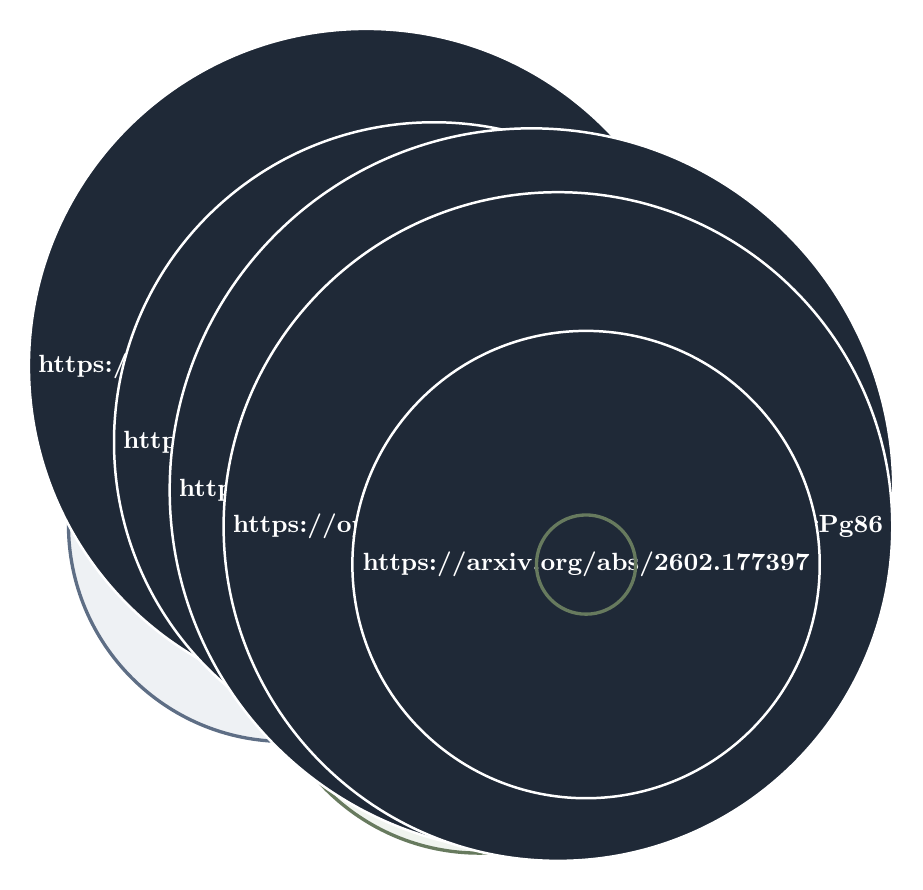
\begin{tikzpicture}[scale=1.05]
  \def\r{2.62}

  % Circle centers
  \coordinate (G) at (-1.30,0.00);
  \coordinate (L) at ( 1.05,1.35);
  \coordinate (A) at ( 1.05,-1.35);

  % Filled circles
  \fill[graphBlue!28, opacity=0.48] (G) circle (\r);
  \fill[llmOrange!34, opacity=0.42] (L) circle (\r);
  \fill[aiGreen!30, opacity=0.44] (A) circle (\r);

  % Outlines
  \draw[line width=1.2pt, graphBlue!75!black] (G) circle (\r);
  \draw[line width=1.2pt, llmOrange!78!black] (L) circle (\r);
  \draw[line width=1.2pt, aiGreen!72!black] (A) circle (\r);

  % Region labels
  \node[font=\bfseries\Large, text=graphBlue!65!black] at (-2.55,0.25) {Graph};
  \node[font=\bfseries\Large, text=llmOrange!72!black, align=center] at (2.25,2.02) {LLM\\/ GFM};
  \node[font=\bfseries\Large, text=aiGreen!65!black] at (2.10,-2.00) {AI4S};

  % Overlap labels
  \node[font=\scriptsize\bfseries, text=ink] at (0.25,2.55) {Graph + LLM};
  \node[font=\scriptsize\bfseries, text=ink] at (2.65,-0.02) {LLM + AI4S};
  \node[font=\scriptsize, text=muted, align=center] at (0.10,0.02) {shared topic\\space};

  % Graph + LLM papers
  \node[
    circle, minimum size=10.8mm, fill=ink, draw=white, line width=0.9pt,
    font=\bfseries\small, text=white
  ] at (-0.32,1.92) {\href{\urlGLEM}{\textcolor{white}{1}}};
  \node[circle, minimum size=12.6mm, draw=graphBlue!70!black, line width=1.2pt] at (-0.32,1.92) {};

  \node[
    circle, minimum size=10.8mm, fill=ink, draw=white, line width=0.9pt,
    font=\bfseries\small, text=white
  ] at (0.08,1.46) {\href{\urlGraphText}{\textcolor{white}{2}}};
  \node[circle, minimum size=12.6mm, draw=graphBlue!70!black, line width=1.2pt] at (0.08,1.46) {};

  \node[
    circle, minimum size=10.8mm, fill=ink, draw=white, line width=0.9pt,
    font=\bfseries\small, text=white
  ] at (0.50,1.00) {\href{\urlGraphAny}{\textcolor{white}{3}}};
  \node[circle, minimum size=12.6mm, draw=graphBlue!70!black, line width=1.2pt] at (0.50,1.00) {};

  % LLM-only paper
  \node[
    circle, minimum size=10.8mm, fill=ink, draw=white, line width=0.9pt,
    font=\bfseries\small, text=white
  ] at (2.30,1.06) {\href{\urlHAX}{\textcolor{white}{4}}};
  \node[circle, minimum size=12.6mm, draw=llmOrange!78!black, line width=1.2pt] at (2.30,1.06) {};

  % LLM + AI4S papers
  \node[
    circle, minimum size=10.8mm, fill=ink, draw=white, line width=0.9pt,
    font=\bfseries\small, text=white
  ] at (1.68,0.42) {\href{\urlPandemicLLM}{\textcolor{white}{5}}};
  \node[circle, minimum size=12.6mm, draw=aiGreen!72!black, line width=1.2pt] at (1.68,0.42) {};

  \node[
    circle, minimum size=10.8mm, fill=ink, draw=white, line width=0.9pt,
    font=\bfseries\small, text=white
  ] at (2.00,-0.02) {\href{\urlRaftPPI}{\textcolor{white}{6}}};
  \node[circle, minimum size=12.6mm, draw=aiGreen!72!black, line width=1.2pt] at (2.00,-0.02) {};

  \node[
    circle, minimum size=10.8mm, fill=ink, draw=white, line width=0.9pt,
    font=\bfseries\small, text=white
  ] at (2.34,-0.48) {\href{\urlGeneZip}{\textcolor{white}{7}}};
  \node[circle, minimum size=12.6mm, draw=aiGreen!72!black, line width=1.2pt] at (2.34,-0.48) {};
\end{tikzpicture}
\end{minipage}
\hfill
\begin{minipage}[t]{0.49\textwidth}
\vspace{0pt}
\RaggedRight
\vspace*{1.15cm}

{\large\bfseries Papers and Links}

\vspace{0.35em}
{\small\color{muted}The same numbering is used in the chart on the left. Each title links directly to the paper.}

\vspace{0.65em}

\paperitem{1}{ICLR23 GLEM}{
  \taglabel{graphBlue}{Graph}\hspace{0.35em}\taglabel{llmOrange}{LLM}
}{\urlGLEM}

\paperitem{2}{arXiv23 GraphText}{
  \taglabel{graphBlue}{Graph}\hspace{0.35em}\taglabel{llmOrange}{LLM}
}{\urlGraphText}

\paperitem{3}{ICLR25 GraphAny}{
  \taglabel{graphBlue}{Graph}\hspace{0.35em}\taglabel{llmOrange}{LLM}
}{\urlGraphAny}

\paperitem{4}{NeurIPS25 HAX}{
  \taglabel{llmOrange}{LLM}
}{\urlHAX}

\paperitem{5}{Nat.\ Comput.\ Sci.\ 25 PandemicLLM}{
  \taglabel{llmOrange}{LLM}\hspace{0.35em}\taglabel{aiGreen}{AI4S}
}{\urlPandemicLLM}

\paperitem{6}{ICLR26 RaftPPI}{
  \taglabel{llmOrange}{LLM}\hspace{0.35em}\taglabel{aiGreen}{AI4S}
}{\urlRaftPPI}

\paperitem{7}{arXiv26 GeneZip}{
  \taglabel{llmOrange}{LLM}\hspace{0.35em}\taglabel{aiGreen}{AI4S}
}{\urlGeneZip}

\vfill

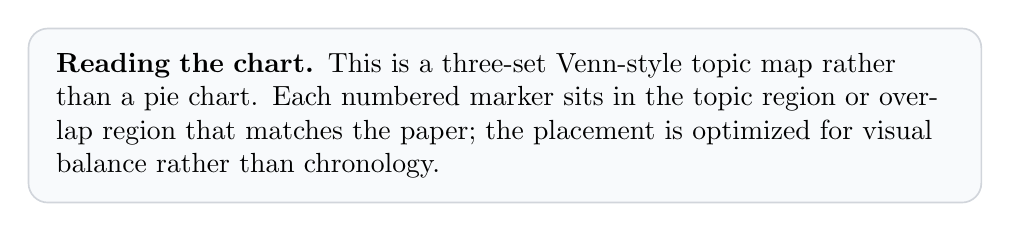
\begin{tikzpicture}
  \node[
    anchor=west,
    rounded corners=7pt,
    fill=panel,
    draw=linegray,
    line width=0.6pt,
    inner xsep=10pt,
    inner ysep=9pt,
    text width=0.94\linewidth
  ] {
    \textbf{Reading the chart.} This is a three-set Venn-style topic map rather than a pie chart. Each numbered marker sits in the topic region or overlap region that matches the paper; the placement is optimized for visual balance rather than chronology.
  };
\end{tikzpicture}

\end{minipage}

\end{document}
